\section{Arduino dengan Infrared Obstacle Detector}
Cara kerja dari Infrared Obstacle Detector yaitu apabila ada penghalang yang menghalangi sinar infrared maka LED notifikasi akan menyala.
\subsection {Code}
Aplikasi penunjang yang kami gunakan dalam membuat code yang akan diterapkan di sensor kami adalah arduino IDE, Berikut adalah code input yang digunakan dalam infrared sensor
\begin {verbatim}
void setup() {
pinMode(A0,INPUT);
pinMode(A1,OUTPUT);
pinMode(A2,OUTPUT);
pinMode(13,OUTPUT);
digitalWrite(A2,HIGH);
digitalWrite(A1,LOW);
Serial.begin(9600);
}
void loop() {
Serial.println(analogRead(A0));
delay(1000);
if(analogRead(A0) < 250){
digitalWrite(13,HIGH);
}
else{
digitalWrite(13,LOW);
}
}
\end{verbatim}

\subsection{Ambil Data}
Ambil data dari uji coba Infrared Obstacle Detector dengan berbagai kertas bewarna, dari mulai delay 1000 sampai delay 100.
 \begin{figure}[!htbp]
  \centering
  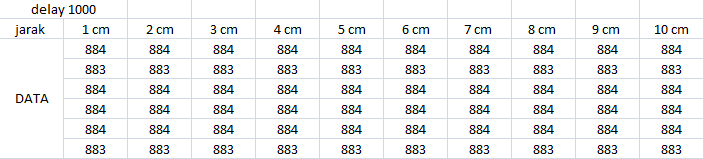
\includegraphics[width=.75\textwidth]{figures/build/delay_1000.png}
  \caption{Saat disetting delay \= 1000}\label{fig:1000}
\end{figure}

 \begin{figure}[!htbp]
  \centering
  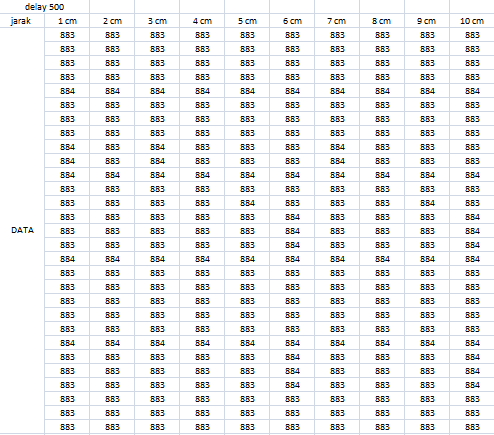
\includegraphics[width=.75\textwidth]{figures/build/delay_500.png}
  \caption{Saat disetting delay \= 500}\label{fig:500}
\end{figure}

 \begin{figure}[!htbp]
  \centering
  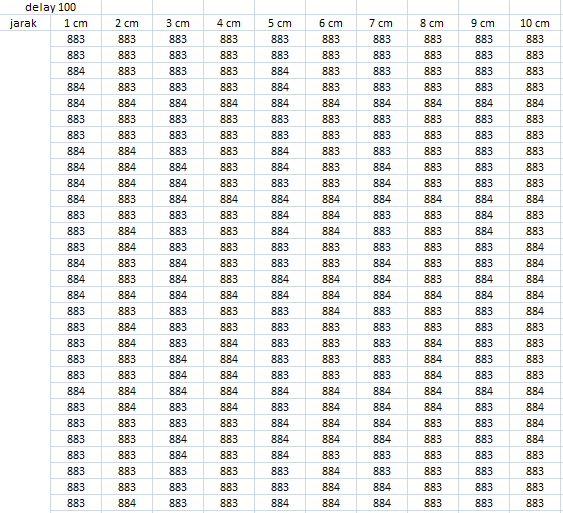
\includegraphics[width=.75\textwidth]{figures/build/delay_100_1.png}
  \caption{Saat disetting delay \= 100 percobaan 1}\label{fig:1001}
\end{figure}

 \begin{figure}[!htbp]
  \centering
  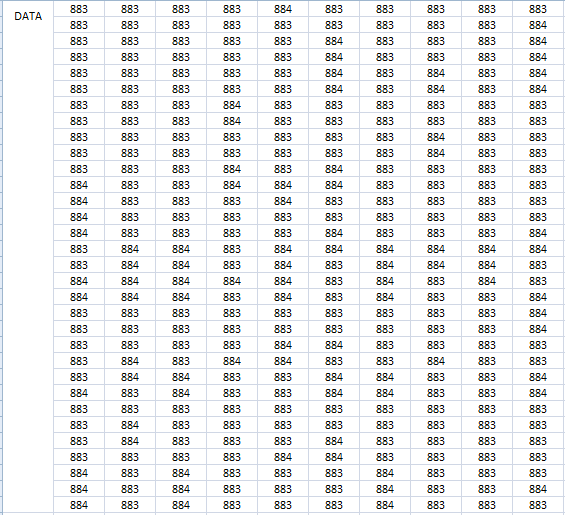
\includegraphics[width=.75\textwidth]{figures/build/delay_100_2.png}
  \caption{Saat disetting delay \= 100 percobaan 2}\label{fig:1002}
\end{figure}